\documentclass{article}

\usepackage{authblk}
\usepackage{graphicx}
\usepackage{array}

\title{
    Comunicação por Computador \\
    \large{Trabalho Prático 1}
}

\author{
    Cristiano Pereira A93726
}

\author{
    Marco Costa A93283
}

\author{
    Hugo Fernandes A89481
}
\date{27 de outubro de 2021}
\affil{
    Universidade do Minho
}

\begin{document}
        \maketitle
    \section*{Respostas}
        \subsection*{Parte I}
            \subsubsection*{1}
                {
                    \centering
                    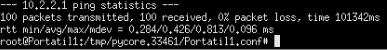
\includegraphics[width=12cm]{images/ping-portatil.png}
                    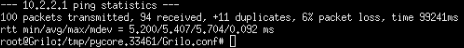
\includegraphics[width=12cm]{images/ping-grilo.png}
                    \par
                }
                    Como podemos ver nas imagens o nó \textit{Grilo}, que no \textit{CORE} lhe foi dada
                uma conexão com 10\% de duplicação e 5\% de packet loss, de 100 pacotes enviados apenas recebeu
                94 mais 11 pacotes duplicados. Isto contrasta com o \textit{Portatil1} que com uma conexão boa conseguiu
                receber os 100 pacotes de resposta sem qualquer duplicação ou perda destes.\par

                    Mais interessante é o resultado destes problemas de conexão no \textit{rtt(round-trip time)} em que se pode verificar
                que o \textit{Grilo} teve valores significativamente mais elevados que a sua contraparte. Apesar disto o \textit{Grilo} demorou
                menos 2101ms a executar.

		Nas aplicações que utillizam TCP na camada de transporte, é a camada de transporte que lida com as perdas e duplicações, ao invés das aplicações que utilizam UDP, onde terá de ser a aplicação a ter este controlo, já que o UDP apenas envia os dados, não verificando a entrega.
            \subsubsection*{2}
                {
                    \centering
                    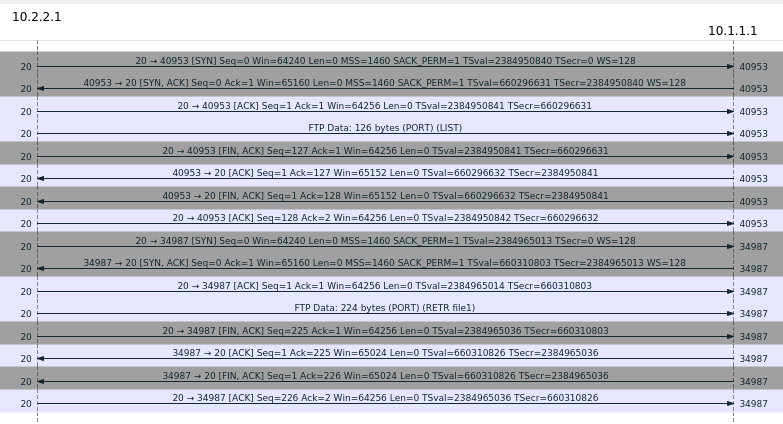
\includegraphics[width=12cm]{images/ftp-flow-graph.png}
                    \par
                }
                    Através do diagrama produzido, pelo Wireshark, podemos ver toda a comunicação FTP feita entre o \textit{Portatil1} (10.1.1.1) e o \textit{Servidor1} (10.2.2.1).

		            O envio do ficheiro entre o servidor e o portátil ocorrem entre as portas 20 e 34987, respetivamente. Os três primeiros segmentos enviados entre estas duas portas correspondem ao inicio da conexão (3-way handshake), o segmento seguinte corresponde à transferência do ficheiro entre as portas, os quatro segmentos finais correspondem à terminação da conexão.

	São utilizados três tipos de segmentos, ACK, FIN e SYN. Os números de sequência utilizados foram 0, 1 e 225 e 226 e os números de ACK 1, 225 e 226.

                    Para além disso, o diagrama mostra que a conexão do lado do servidor está a ser feita na porta 20 que é reservada para o protocolo FTP.
            \subsubsection*{3}
                {
                    \centering
                    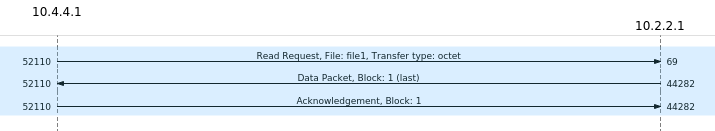
\includegraphics[width=12cm]{images/tftp-wireshark-flow-graph.png}
                    \par
                }
		            Através do diagrama produzido, pelo Wireshark, podemos ver toda a comunicação TFTP feita entre o \textit{Portatil1} (10.1.1.1) e o \textit{Servidor1} (10.2.2.1).

                    O protocolo TFTP mostra-se bem mais simples que o FTP, tendo sido apenas trocados 3 segmentos, pois utiliza UDP na camada de transporte o que significa que não tem as fases de início e fim de conexão.

                    É feito um \textit{Read Request}, o servidor envia o ficheiro e, por fim, o portátil responde com um \textit{Acknowledgement}.

                    Tal como no exercício anterior podemos conferir no diagrama que o servidor inicia a conexão na porta 69 que corresponde a porta reservada para o TFTP. No entanto, a conexão muda para a porta 44209 para ocorrer a transferência do ficheiro.
            \subsubsection*{4}
		            Em relação à camada de transporte, a aplicação TFTP é a única que utiliza UDP, o que lhe uma vantagem na velocidade de transmissão. As restantes aplicações utilizam TCP, no entanto versões mais recentes de HTTP utilizam UDP+QUIC.

                    Após o uso dos quatro programas podemos concluir que o mais seguro é o sftp pelo seu uso do protocolo ssh que encripta toda a comunicação entre despositivos. Enquanto que FTP e TFTP não fazem encriptação nenhuma dos dados.

                    De todos os serviços utilizados o SFTP é o mais complexo devido à encriptação dos dados que, em conjunto com o uso de TCP, criam um \textit{overhead} forte, tornando este protocolo o mais pesado, e,  consequentemente, o mais lento. Inversamente, o TFTP mostra-se o mais simples 
                pelo seu uso do protocolo UDP. Assim, todo o processo de deteção de erros passa para a camada da aplicação, o que permite remover toda a complexidade que o TCP trás consigo que o TFTP não precisa.
                
                    Finalmente, o HTTP oferece uma alternativa aos restantes protocolos pela informação extra que carrega face aos outros protocolos, mas peca pelo overhead que essa informação introduz, bem como pela transparência desta.  
        \subsection*{Parte II}
            \begin{center}
                \scalebox{0.6}{
                    \begin{tabular}{|m{2.8cm}|m{4.1cm}|m{4.3cm}|m{3.8cm}|m{3.5cm}|}
                        \hline
                        \textbf{Comando usado (aplicação)} & \textbf{Protocolo de Aplicação (se aplicável)} & \textbf{Protocolo de Transporte (se aplicável)} & \textbf{Porta de atendimento (se aplicável)} & \textbf{\textit{Overhead} de transporte em bytes (se aplicável)} \\
                        \hline
                        ping          & Não tem   & Não tem & Não tem          &  0 \\
                        \hline
                        traceroute    & Não tem   & Não tem & Não tem          &  0 \\
                        \hline 
                        telnet        & telnet & tcp     & 23               & 20*nºseg + 74*nº[SYN,ACK] + 66*nº[FIN,ACK] \\
                        \hline
                        ftp           & ftp    & tcp     & 20,21            & 20*nºseg + 74*nº[SYN,ACK] + 66*nº[FIN,ACK] \\
                        \hline
                        tftp          & tftp   & udp     & 69, Aleatório    &  8*nºseg \\
                        \hline
                        http(browser) & http   & tcp     & 80               & 20*nºseg + 74*nº[SYN,ACK] + 66*nº[FIN,ACK] \\
                        \hline
                        nslookup      & dns    & udp     & 53               &  8*nºseg \\
                        \hline
                        ssh           & ssh    & tcp     & 22               & 20*nºseg + 74*nº[SYN,ACK] + 66*nº[FIN,ACK] \\
                        \hline
                    \end{tabular}
                }
            \end{center}
        \clearpage
        \subsection*{Conclusões}
                Com a conclusão do Trabalho Prático 1 tornam-se claros os seus propósitos de consolidar a matéria referente aos protocolos da camada de transporte (TCP e UDP), várias aplicações de transferência de serviços e as suas vantagens e desvantagens, bem como a introdução a outros conceitos e ferramentas importantes para futuro da UC. Destes, destacam-se o primeiro contacto com o CORE e o Wireshark. 
                
\end{document}